Let \(s = \frac{\log 3}{\log 2}\). We restate some definitions first: let \(I_n = (i_1, i_2, \ldots, i_n) \in \{1, 2, 3\}^n\) where \(i_k \in \{1, 2, 3\}\) for each \(1 \leq k \leq n\), and define \(S_{I_n}(\Delta) = S_{i_1}(S_{i_2}(\ldots(S_{i_n}(\Delta))))\) where \(\Delta\) is the closed equilateral triangle with vertices \((0, 0), (1, 0)\) and \(\left(\frac{1}{2}, \frac{\sqrt{3}}{2}\right)\).

We define for \(E \subset \R^2\) that
\[
S(E) = \bigcup_{i = 1}^{3} S_i(E).
\]

\begin{itemize}
    \item \textbf{Upper Bound: \(\h^s(\sierpinski) \leq  1\).} Recall the definition that
    \[
    \h^s_\delta(\sierpinski) = \inf_{\{U_i\} \text{ is a }\delta\text{-cover of }\sierpinski} \sum_{i = 1}^{+\infty} |U_i|^s.
    \]

    We can first show that \(|\triangle| \geq 1\) since \(|(0, 0) - (1, 0)| = 1\) and \(|\triangle| \leq 1\) since \(\triangle \subset \overline{B_{(0, 0)} (1)}\). And therefore, we can see that
    \[
    \left|S_{I_n}(\triangle)\right| = \frac{1}{2^n}
    \]
    from the definition of a contraction immediately.

    By theorem 4.0.2, we can see that
    \[
        \sierpinski = \bigcap_{k = 0}^{+\infty} S^{(k)}(\Delta)
    \]
    since \(\sierpinski\) is the attractor of the IFS.

    Consider a certain \(k \in \Z, k \geq 0\), and it is not difficult to see from definition that
    \[
        S^{(k)} (\Delta) = \bigcup_{I_n \in \{1, 2, 3\}^n} S_{I_n} (\Delta)
    \]
    from the definition of \(S^{(k)}\). (This can be shown by induction on \(k\).)

    Therefore, we can see
    \[
        \sierpinski \subset \bigcup_{I_n \in \{1, 2, 3\}^n} S_{I_n} (\Delta),
    \]
    and therefore, \(\{S_{I_n} (\Delta)\}\) gives a \(\delta\)-cover for \(\sierpinski\), when \(\delta > \frac{1}{3^n} \iff 3^n > \frac{1}{\delta} \iff n > -\log_3(\delta)\).

    Also, notice that \(\# \{S_{I_n} (\Delta)\} = 3^n\).

    Therefore, for any \(0 < \delta < 1\), choose \(n = \floor{-\log_3(\delta)} + 1 \implies n > -\log_3(\delta)\), and therefore
    \begin{align*}
        \h^s_\delta(\sierpinski) &= \inf_{\{U_i\} \text{ is a }\delta\text{-cover of }\sierpinski} \sum_{i = 1}^{+\infty} |U_i|^s\\
        &\leq \sum_{i = 1}^{3^n} \left(\frac{1}{2^n}\right)^{s}\\
        &= 3^n \cdot \frac{1}{2^{\left(n \cdot \log_2(3)\right)}}\\
        &= 3^n \cdot \frac{1}{3^n}\\
        &= 1,
    \end{align*}
    and therefore
    \[
        \h^s(\sierpinski) = \lim_{\delta \to 0} \h^s_\delta(\sierpinski) \leq 1,
    \]
    which shows the upper bound as desired.

    \item We show that the IFS of the Sierpinski triangle satisfies the OCS. Consider the open set \(U\) which is the open triangle with vertices \((0, 0), (1, 0), \left(\frac{1}{2}, \frac{\sqrt{3}}{2}\right)\). We notice that
    \begin{align*}
        S_1(U) &\text{ is an open triangle with vertices } (0, 0), \left(\frac{1}{2}, 0\right), \left(\frac{1}{4}, \frac{\sqrt{3}}{4}\right),\\
        S_2(U) &\text{ is an open triangle with vertices } \left(\frac{1}{2}, 0\right), \left(1, 0\right), \left(\frac{3}{4}, \frac{\sqrt{3}}{4}\right),\\
        S_3(U) &\text{ is an open triangle with vertices } \left(\frac{1}{4}, \frac{\sqrt{3}}{4}\right), \left(\frac{3}{4}, \frac{\sqrt{3}}{4}\right), \left(\frac{1}{2}, \frac{\sqrt{3}}{2}\right),
    \end{align*}
    and therefore they are pairwise disjoint and are all subsets of \(U\). Therefore the IFS satisfies the open set condition.
    
    Now, we show that the natural measure on \(\sierpinski\) satisfies the hypothesis for the mass distribution principle, for \(\epsilon = 1\) and \(c = 6\).

    Consider some \(U \subset \sierpinski\) such that \(|U| < 1\). There must exist some \(k\) such that \(2 \cdot 2^{-(k+1)} \leq |U| < 2 \cdot 2^{-k}\) for some \(k \geq 1\). Then, \(U \subset \bigcup_{i = 1}^{6} \left(\Delta_{k}\right)_i \cap \sierpinski\), where \(\Delta_{t}\) is a triangle formed in the \(t\)'s iteration of the IFS. This means that \(U\) is in at most \(6\) triangles in the \(k\)-th iteration, as shown in the diagram below:

    \begin{center}
        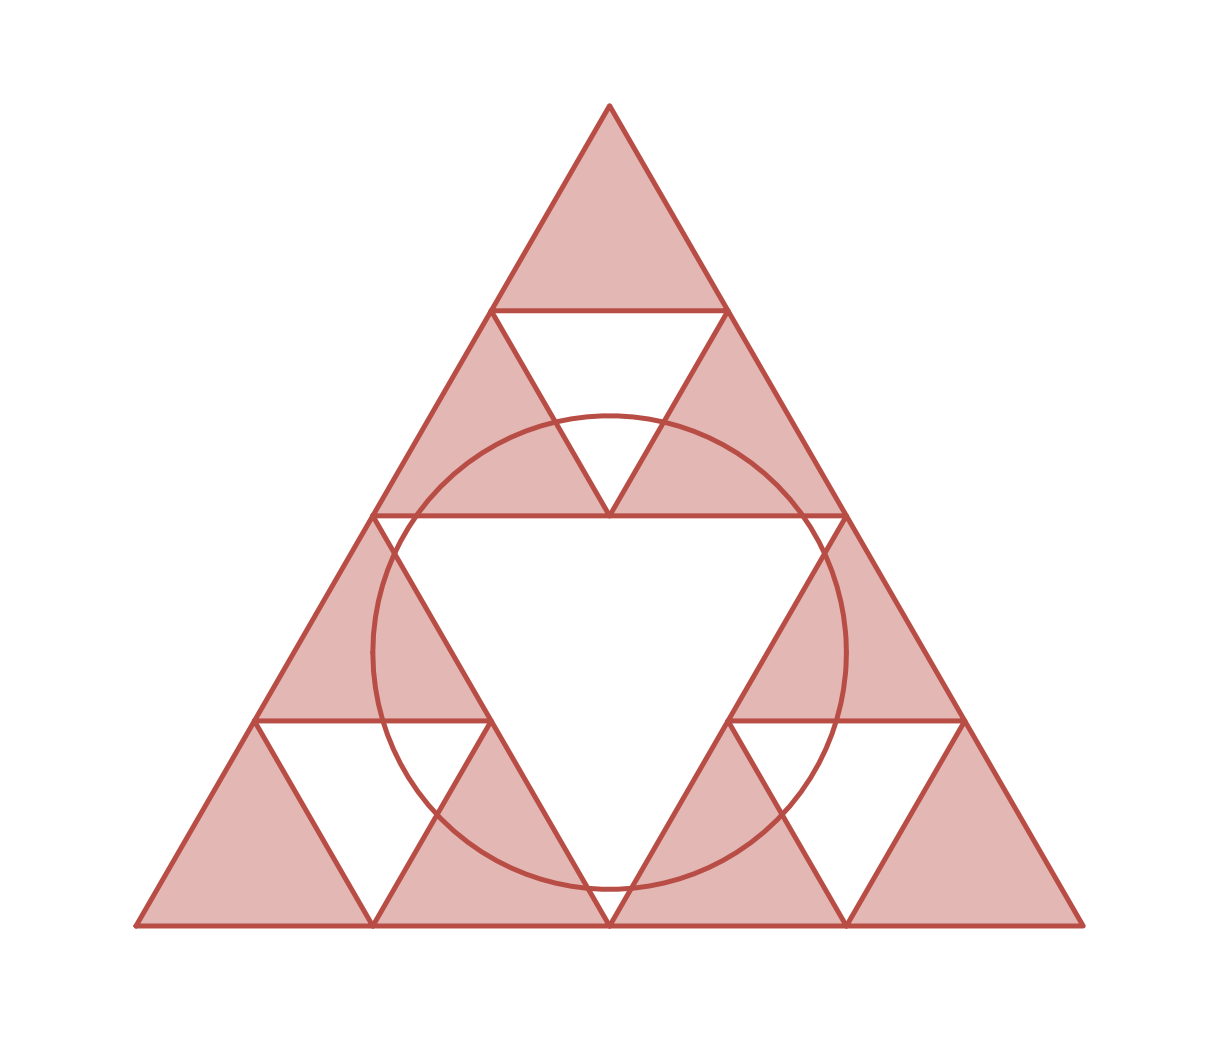
\includegraphics[scale=0.4]{solutions/section-5-0/diag-5-0-1.png}
    \end{center}
    
    Therefore we will have

    \begin{align*}
        \mu(U) & \leq 2 \cdot 3^{-k}\\
        &= 6 \cdot \left(2^{\log_2^3}\right)^{-(k+1)}\\
        &= 6 \cdot \left(2^{-(k+1)}\right)^{\log_2^3}\\
        &\leq 6 \cdot |U|^s.
    \end{align*}

    Notice that \(\mu(\sierpinski) = \mu(\Delta \cap \sierpinski) = \mu(S_{I_0} (\Delta) \cap \sierpinski) = 1\) and therefore,
    \[
    \h^s(\sierpinski) \geq \frac{\mu(\sierpinski)}{6} = \frac{1}{6}
    \]
    as desired.
\end{itemize}